\subsection{Figuring the Move Order based on pick outcome}

On guessing with some certainty the move order from the pick outcome in non-light fog templates. examples from inss, or templates with a lot of picks, where you can be somewhat certain what the move order is based on the picks. Not 100\% but somewhat certain. 
\\
\\
For example in this \href{https://www.warzone.com/MultiPlayer?GameID=40500155}{Earthsea} game at Figure \ref{earthsea} (my picks are pretty bad, don't use this as a guideline for how to pick on the template), I receive 1/2/4/7/8 and lose 3/5/6 as well 10. The issue after the territory allocation is that without information on the move order, I cannot make sound moves as me and Guest are contesting two red +1 castles.

\begin{figure}[H]
  \centering
  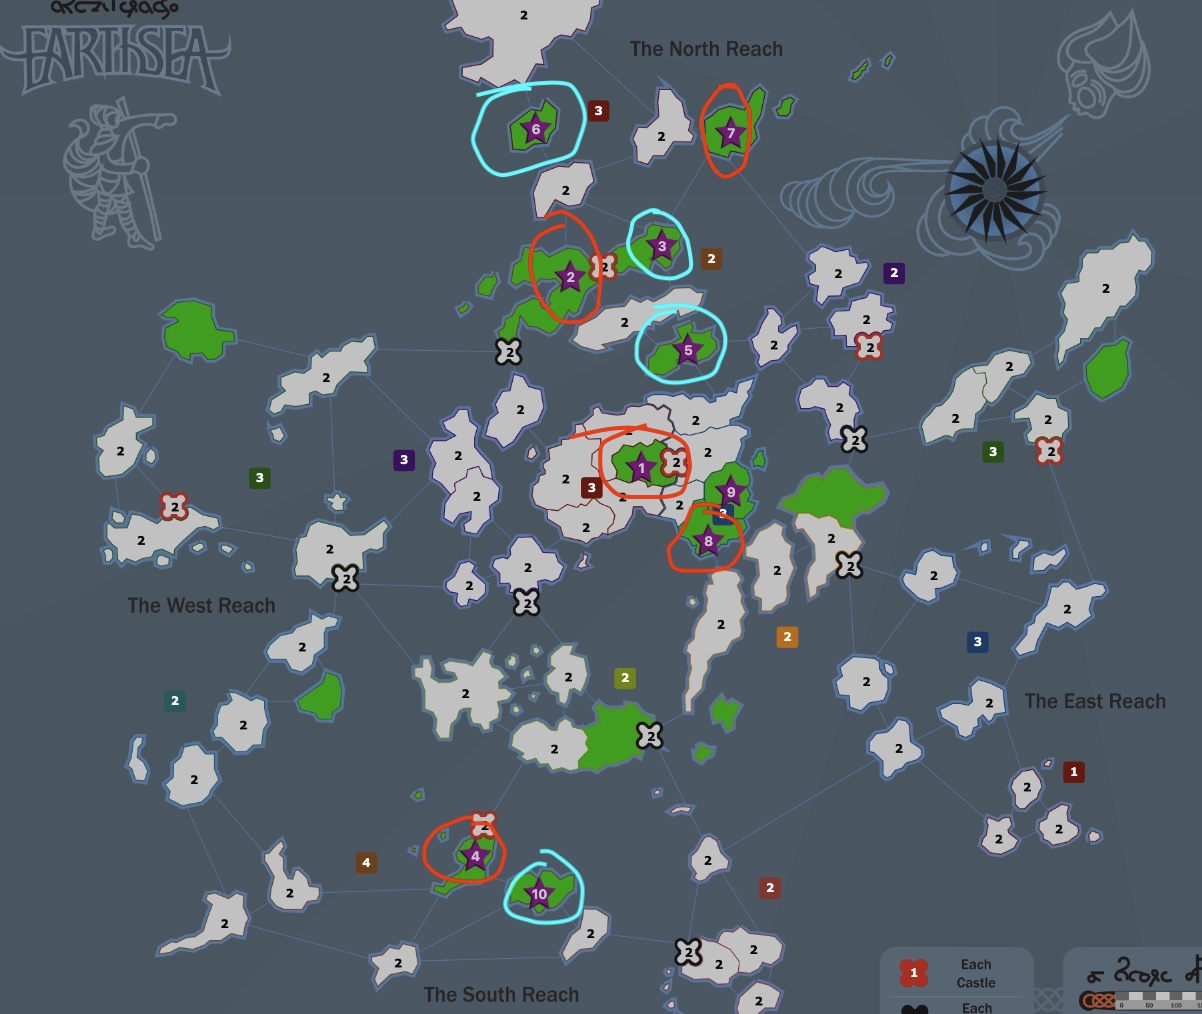
\includegraphics[width=0.7\textwidth]{Images/earthsea.jpg}
  \caption{My picks. Red circle what I received. Light Blue circle what I lost and what I have vision on.}
  \label{earthsea}
\end{figure}

But let's assume that I was first pick, meaning Guest moves first on turn 1. Then the allocation would have to look like \ref{earth_guest} which logically speaking doesn't make sense from any possible perspective.  With the numbers below identifying the territories as I picked them:
\begin{itemize}
    \item If Guest decided to include all the territories that border the +1s, or 3/4 of those, in his first 4 picks, it is impossible for me get 3/4 as first pick. It would have to be 7ate9: 1, Guest: 2,3, 7ate9: 4,5 etc but I received 1,2,4.
    \item If Guest decided to do picks in order of 1->2->3->5 prioritising the central +1 followed by the ftb I picked at 2/3/5, or did his first three picks on my 2/3/5, it again doesn't make sense.
\end{itemize}

It is useful in your own games to try and apply trial and error into thinking what was your opponents idea in picks so as to derive how they will act upon the distribution they received, as well as the move order. In this game, while I am not certain of the move order, I am fairly confident I was second pick and choose to play my moves under that assumption.

\begin{figure}[H]
  \centering
  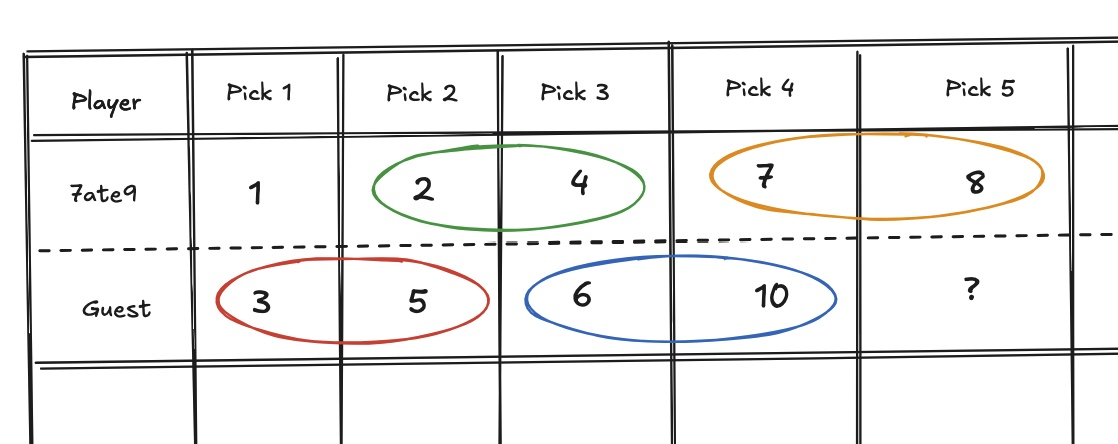
\includegraphics[width=0.7\textwidth]{Images/earhsea_oucome.jpg}
  \caption{For move order: 1. 7ate9, 2. Guest on picks}
  \label{earth_guest}
\end{figure}